\documentclass[12pt,]{article}
\usepackage[left=1in,top=1in,right=1in,bottom=1in]{geometry}
\newcommand*{\authorfont}{\fontfamily{phv}\selectfont}
\usepackage{lmodern}


  \usepackage[T1]{fontenc}
  \usepackage[utf8]{inputenc}



\usepackage{abstract}
\renewcommand{\abstractname}{}    % clear the title
\renewcommand{\absnamepos}{empty} % originally center

\renewenvironment{abstract}
 {{%
    \setlength{\leftmargin}{0mm}
    \setlength{\rightmargin}{\leftmargin}%
  }%
  \relax}
 {\endlist}

\makeatletter
\def\@maketitle{%
  \newpage
%  \null
%  \vskip 2em%
%  \begin{center}%
  \let \footnote \thanks
    {\fontsize{18}{20}\selectfont\raggedright  \setlength{\parindent}{0pt} \@title \par}%
}
%\fi
\makeatother




\setcounter{secnumdepth}{0}


\usepackage{graphicx}
% We will generate all images so they have a width \maxwidth. This means
% that they will get their normal width if they fit onto the page, but
% are scaled down if they would overflow the margins.
\makeatletter
\def\maxwidth{\ifdim\Gin@nat@width>\linewidth\linewidth
\else\Gin@nat@width\fi}
\makeatother
\let\Oldincludegraphics\includegraphics
\renewcommand{\includegraphics}[1]{\Oldincludegraphics[width=\maxwidth]{#1}}

\title{Inaction on climate change could cost one year of life in some European
countries \thanks{All data and code that supports these conclusions are available as
supplementary materials. The authors would like to thank E. Carlson for
his helpful comments.}  }



\author{\Large Mathew E. Hauer\textsuperscript{1,2}*\vspace{0.05in} \newline\normalsize\emph{Florida State University}   \and \Large Alexis R. Santos\textsuperscript{3}\vspace{0.05in} \newline\normalsize\emph{Pennsylvania State University}  }


\date{}

\usepackage{titlesec}

\titleformat*{\section}{\normalsize\bfseries}
\titleformat*{\subsection}{\normalsize\itshape}
\titleformat*{\subsubsection}{\normalsize\itshape}
\titleformat*{\paragraph}{\normalsize\itshape}
\titleformat*{\subparagraph}{\normalsize\itshape}





\newtheorem{hypothesis}{Hypothesis}
\usepackage{setspace}

\makeatletter
\@ifpackageloaded{hyperref}{}{%
\ifxetex
  \PassOptionsToPackage{hyphens}{url}\usepackage[setpagesize=false, % page size defined by xetex
              unicode=false, % unicode breaks when used with xetex
              xetex]{hyperref}
\else
  \PassOptionsToPackage{hyphens}{url}\usepackage[unicode=true]{hyperref}
\fi
}

\@ifpackageloaded{color}{
    \PassOptionsToPackage{usenames,dvipsnames}{color}
}{%
    \usepackage[usenames,dvipsnames]{color}
}
\makeatother
\hypersetup{breaklinks=true,
            bookmarks=true,
            pdfauthor={Mathew E. Hauer\textsuperscript{1,2}* (Florida State University) and Alexis R. Santos\textsuperscript{3} (Pennsylvania State University)},
             pdfkeywords = {Climate change, Life expectancy, Mortality, Demography, Excess
mortality, Europe, Public health},  
            pdftitle={Inaction on climate change could cost one year of life in some European
countries},
            colorlinks=true,
            citecolor=blue,
            urlcolor=blue,
            linkcolor=magenta,
            pdfborder={0 0 0}}
\urlstyle{same}  % don't use monospace font for urls

\usepackage[all]{nowidow}
\usepackage{rotating}
\usepackage{fancyhdr}
\usepackage[table]{xcolor}
\usepackage{tabularx}
\usepackage{makecell}
\usepackage{xcolor}
\pagestyle{fancy}
\fancyhead{}
\fancyhead[C]{Climate change life expectancy}


% add tightlist ----------
\providecommand{\tightlist}{%
\setlength{\itemsep}{0pt}\setlength{\parskip}{0pt}}

\begin{document}
	
% \pagenumbering{arabic}% resets `page` counter to 1 
%
% \maketitle

{% \usefont{T1}{pnc}{m}{n}
\setlength{\parindent}{0pt}
\thispagestyle{plain}
{\fontsize{18}{20}\selectfont\raggedright 
\maketitle  % title \par  

}

{
   \vskip 13.5pt\relax \normalsize\fontsize{11}{12} 
\textbf{\authorfont Mathew E. Hauer\textsuperscript{1,2}*} \hskip 15pt \emph{\small Florida State University}   \par \textbf{\authorfont Alexis R. Santos\textsuperscript{3}} \hskip 15pt \emph{\small Pennsylvania State University}   

}

}








\begin{abstract}

    \hbox{\vrule height .2pt width 39.14pc}

    \vskip 8.5pt % \small 

\noindent Climate change-related excess mortality estimates clearly demonstrate a
dramatic impact on public health and human mortality. However, life
expectancy at birth is more easily communicated and understood by the
public. By properly situating climate change mortality within the
contexts of life expectancy, we better represent the cost of climate
change on longevity. In this paper, we convert excess mortality
estimates due to increases in extreme weather from climate change into
potential reductions in life expectancy at birth in twenty-eight
European countries. We project climate change extremes to reduce life
expectancy at birth by 0.24 years for the average European country with
differences in excess of 1.0 years in some countries by 2100. We only
estimate the impact of mortality directly related to climate extremes,
making our estimates conservative. Thus, the cost of inaction on climate
change could approach, and likely to exceed, one year of life in some
European countries.


\vskip 8.5pt \noindent \emph{Keywords}: Climate change, Life expectancy, Mortality, Demography, Excess
mortality, Europe, Public health \par

    \hbox{\vrule height .2pt width 39.14pc}



\end{abstract}


\vskip 6.5pt


\noindent \doublespacing \begin{itemize}
\tightlist
\item
  Corresponding author.
  \href{mailto:mehauer@fsu.edu}{\nolinkurl{mehauer@fsu.edu}} p:
  850-644-7103.
\end{itemize}

\textsuperscript{1} Department of Sociology, Florida State University.
113 Colleggiate Way, Bellamy Building, Tallahassee FL 30602.

\textsuperscript{2} Center for Demography and Population Health, Florida
State University.

\textsuperscript{3} Department of Sociology and Criminology,
Pennsylvania State University. 901 Oswald Tower, University Park, PA USA
16802.

\newpage

\hypertarget{main-text}{%
\section{Main Text}\label{main-text}}

Climate change's implications on humanity go far beyond estimates of
economic damages (Hsiang et al. 2017), estimates of displacement (Rigaud
et al. 2018), or human conflict (Barnett and Adger 2007) but have the
potential to contribute to the loss of human life (Forzieri et al. 2017;
Pachauri et al. 2014). As impact quantification studies move further
from the physical sciences of climate change, properly quantifying and
conveying the impact of climate change on public health is of increasing
importance (Cloyd et al. 2016; Melillo, Richmond, and Yohe 2014).

Scholars have long estimated the mortality risks associated with climate
change and typically use excess or extra mortality (Forzieri et al.
2017; McMichael, Woodruff, and Hales 2006; Wilson et al. 2017; Zanobetti
et al. 2012). For example, Forzieri et al. (2017) projected climate
change extremes to increase European mortality by 150,000+ persons per
year by the end of the century. Although such estimates are useful, the
excess mortality estimates are rather sterile -- one death is a tragedy,
a million deaths a statistic -- and difficult to relate to on a personal
level. Life expectancy at birth (\(e_0\)), on the other hand, provides
potent comparisons of mortality vectors and converts excess mortality
into an intuitively understood metric, relatable to everyone. To our
knowledge, no studies exist that comprehensively examine the potential
reductions of life expectancy due to climate change. Without properly
situating the potential loss of life within the contexts of metrics such
as life expectancy, we risk underestimating the impact of climate change
on human mortality.

Using published data on excess mortality (Forzieri et al. 2017), we
connect climate change excess mortality to life expectancy in a
mortality model. By estimating the increase in age-specific mortality
rates associated with previously published excess death estimates, we
can assess how much climate change could reduce the anticipated
longevity of the average person in twenty-eight European countries. This
approach allows us to quantify the impact of climate change on human
longevity and answer the following question: What is the cost of
inaction on climate change on human longevity? Our results situate
climate change mortality within the broader context of human mortality
and can be used to inform public health interventions to prevent such
futures.

Our results suggest that climate change could emerge as a potent public
health threat in the 20th century. Mitigation strategies (ie reductions
in greenhouse gas emisions) and adaptation strategies (ie outreach
efforts, retrofitting public buildings, etc.) would help prevent this
new public health concern.

\hypertarget{methods-and-materials}{%
\section{Methods and Materials}\label{methods-and-materials}}

\hypertarget{data}{%
\subsection{Data}\label{data}}

We estimate changes in life expectancy by combining three primary
datasets: excess mortality data due to meterological hazards related to
climate change from Forzieri et al. (2017), cause-of-death distributions
from the Global Burden of Disease study (GBD) (Disease Study 2015 2017;
Wang et al. 2012), and life tables from the Human Mortality Database
(HMD) (Database 2017).

Forzieri et al. (2017) combined data from the International Disaster
Database (EMCAT) and the Natural Catastrophe Statistics tool
(NatCatSERVICE) to create exposure and fatality statistics related to
six weather-related hazards -- heatwaves, cold waves, droughts,
wildfires, river and coastal floods, and windstorms -- and estimated
excess mortality associated with those hazards during a baseline period
of 1981-2010 in 28 European countries. They only considered fatalities
\emph{directly attributable} to the event and \emph{exclude} increased
deaths from common causes that were observed to rise during the event,
such as cardiovascular or respiratory deaths\footnote{``The fatality
  data from the two databases considered is likely to not include
  increased deaths from common causes that were observed to rise at the
  population level but for which individual deaths could not be
  attributed to the event. For example,\ldots{} increased risk of
  cardiovascular and respiratory deaths \ldots{} may be severly
  underreported in the EMDAT and NatCatSERVICE.'' (see Forzieri et al.
  2017:9, \emph{Supplementary Materials}).}. While the disaster data are
not standardized across country, Forzeri et al.~imputed data in
incomplete time periods and countries. This imputation could mask
spatial variability at the sub-national level, but here we use their
country-aggregated results. They downscaled these exposures rates to 1km
grid cells and integrated them into small-area demographic projections
for Europe out to 2100 that correspond to a middle-of-the-road
socioeconomic scenario (SSP2 with medium fertility, medium mortality,
medium migration, and the Global Education Trend education scenario
(Jiang 2014; O'Neill et al. 2017; Samir and Lutz 2017)) and based their
projected mortality on extrapolations of their calculated exposures.
Their results represent business-as-usual climate change and human
development without incorporating potential adaptations to climate
change. They found a potential 150,000+ climate change related
fatalities per year by the mid 2080s with climate change contributing to
90\% of mortality rise as opposed to population changes. The number of
future anticipated deaths are available in their Supplementary Table S8
(Forzieri et al. 2017) and provide the magnitude of deaths for our
study.

\begin{figure}
\centering
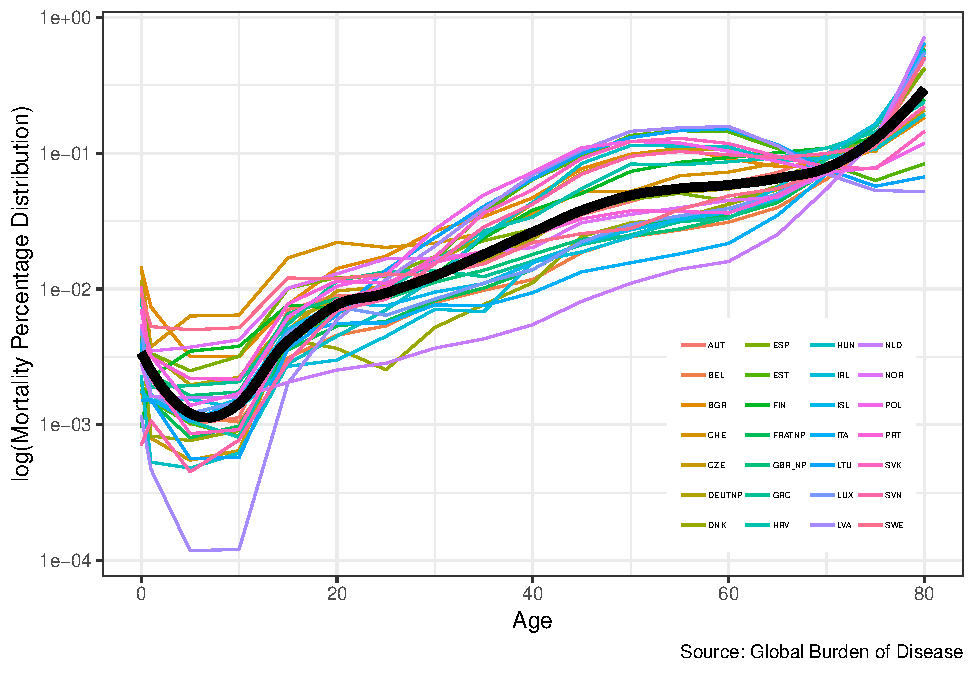
\includegraphics{MS-cclifeexpec_files/figure-latex/suppfig-1.pdf}
\caption{\textbf{Mortality distribution of Heat-related mortality in 28
European countries}. The thick black line is the average\label{suppfig}}
\end{figure}

The Forzieri et al. (2017) data contain only mortality totals and report
no age detail, precluding a direct conversion from excess mortality to
life expectancy. To convert excess mortality to life expectancy, we
allocate excess multi-hazard mortality for each country based on the
observed age-specific mortality schedule for environmental heat and cold
exposure deaths from the GBD (Disease Study 2015 2017; Wang et al.
2012). Forzieri et al.~found that extreme heat (as opposed to other five
weather-related hazards) account for 99\% of the anticipated excess
mortality by the end of the century. The GBD is the most comprehensive
worldwide dataset of epidemiological data produced and provides
cause-specific mortality by age/sex/geography/year for 249 causes of
death in 195 countries and territories. We gathered data on age-specific
deaths and mortality rates (\(m_x\)) for mortality from environmental
heat and cold exposure (cause C.2.9) for the period 2006-2015 for each
country in the study. These data provide a mortality schedule to fit the
projected climate change excess mortality from Fozieri et al (Forzieri
et al. 2017). Thus, we assume that the age-specific mortality schedules
observed between 2006 and 2015 due to environmental heat and cold
exposure in the GBD (see \autoref{suppfig}) are likely to remain
unchanged in the future. We only use the GBD to distribute the Forzieri
et al.~deaths by age.

With the Forzier et al data and the GBD we estimate the anticipated
age-specific mortality schedules due to climate change in twenty-eight
European countries but we cannot compare life expectancy differentials
in the absence of Climate Change using those two datasets alone. To
create baseline mortality schedules and life expectancy, we gather data
from the Human Mortality Database (Database 2017) for the corresponding
European countries. The HMD comprises only complete, official vital
event statistics and represents the most accurate and complete
compilation of mortality data available. We downloaded the most recent
5x1 (age by year) life table data for the twenty-eight European
countries (see \autoref{Table2} for a list of countries and most recent
mortality data).

\begin{table}
\caption{\textbf{Most recent mortality data available by country in the HMD.}} \label{Table2}
\begin{tabular}{ll|ll|ll|ll}
Country & Year & Country & Year & Country & Year & Country & Year \\
\hline
AUT     & 2014 & ESP     & 2014 & HUN     & 2014 & NLD     & 2016 \\
BEL     & 2015 & EST     & 2014 & IRL     & 2014 & NOR     & 2014 \\
BGR     & 2010 & FIN     & 2015 & ISL     & 2016 & POL     & 2014 \\
CHE     & 2016 & FRATNP  & 2015 & ITA     & 2014 & PRT     & 2015 \\
CZE     & 2016 & GBR     & 2016 & LTU     & 2014 & SVK     & 2014 \\
DEUT    & 2015 & GRC     & 2013 & LUX     & 2014 & SVN     & 2014 \\
DNK     & 2016 & HRV     & 2016 & LVA     & 2014 & SWE     & 2016 \\
\hline
\end{tabular}
\end{table}

We used the following data elements from the five-year age group life
table data in the HMD:

\begin{enumerate}
\item $_nP_x$ or the population in age group $x$ for $n$-year intervals from exact age $x$ to $x+n$.
\item $_na_x$ or the average length of survival between ages $x$ and $x+n$.
\item $_nd_x$ or the number of deaths in age group $x$ for $n$-year intervals from exact age $x$ to $x+n$.
\end{enumerate}

\hypertarget{methods}{%
\subsection{Methods}\label{methods}}

We derived a number of additional variables to accomplish our analysis.
First, we abridged the life table data from the HMD from ages 100+ to
80+ to conform to the GBD cause-specific mortality schedules.

From the GBD data, we derived variable \(t_{x,i}\) as the proportion of
deaths, \(D\), from each age group \(x\) in each country \(i\)
(\(_nt_{x,i}=D_{x,i}^{GBD}/\sum_{\alpha=0}^{80}{_nD_{\alpha,i}^{GBD}}\)).

We then derived additional \(m_x\) rates for each age group \(x\) in
each country \(i\) for each scenario \(s\) (\(BASE\), \(LOW\), \(MID\),
\(HIGH\)) from Forzieri et al (Forzieri et al. 2017).

\begin{equation}
_nm_{x,i,BASE} = _nD_{x,i}^{HMD} \,/\, _nP_{x,i}^{HMD}
\end{equation}

\begin{equation}
_n\hat{m}_{x,i,s} = (_nD_{x,i}^{HMD} + (\hat{D_{i,s}} \,\cdot\, _nt_{x,i}) ) \,/\, _nP_{x,i}^{HMD}
\end{equation}

where \(D_{x,i}\) is the number of deaths in age group \(x\) in country
\(i\) from the HMD, \(P_{x,i}\) is the population in age group \(x\)
from the HMD, \(\hat{D_{i,s}}\) is the number of deaths from Forzieri et
al. (Forzieri et al. 2017) under scenario s, and \(t_{x,i}\) is the
proportion of mortality experienced in each age group \(x\) from the
GBD. Thus, the anticipated additional mortality due to climate change is
added to each age group based on the underlying cause-specific mortality
schedule observed between 2006-2015 in the GBD.

We then calculated \(q_x\) values, or the probability of dying, for each
scenario \(s\) for each country.

\begin{equation}
_nq_{x,i,BASE} = \frac{m_{x,i,BASE}}{1+(n-_na_{x,i}) \cdot m_{x,i,BASE}}
\end{equation}

\begin{equation}
_n\hat{q}_{x,i,s} = \frac{\hat{m}_{x,i,s}}{1+(n-_na_{x,i}) \cdot \hat{m}_{x,i,s}}
\end{equation}

We calculated each additional life table value identically for each
scenario \(s\) using standard life table equations:

\[_nd_{x,i,s} = _nl_{x,i,s} \cdot _nq_{x,i,s}\]
\[_nl_{x,i,s} = _nl_{x-1,i,s} - _nd_{x-1,i,s}\]
\[_nL_{x,i,s} = _na_{x,i,s} \cdot _nl_{x,i,s} + ((n-_na_{x,i,s}) \cdot _nl_{x,i,s})\]
\[_nT_{x,i,s} = _nL_{x,i,s} + _nT_{x+1,i,s}\]
\[_ne_{x,i,s} = _nT_{x,i,s} / _nl_{x,i,s}\]

To determine the differences between life expectancy compared to the
baseline, we simply subtract \(e_{x,i,s}\) (for scenario \(LOW\),
\(MID\), and \(HIGH\)) from \(e_{x,i,BASE}\) as described by
(Beltrán-Sánchez, Preston, and Canudas-Romo 2008).Complete life tables
for all countries are available in the \emph{Supplementary Dataset} and
all computer code to replicate our results are available
online\footnote{Replication files are located here:
  \url{https://osf.io/fp52x/?view_only=754d9a72a2ea4f6b8e0c193dc9a590d1}}.

\hypertarget{results}{%
\section{Results}\label{results}}

We find that climate change could alter life expectancy by -0.23 years
(-2.5 months (-0.1 to -0.39 years)) in the average European country
(\textbf{\autoref{figure1}}) by 2100. This reduction is comparable to
mortality due to influenza and pneumonia (Arias, Heron, and Tejada-Vera
2013) in the United States for the year 2000. Although the average
European country could see a change of -0.23 years, several countries
are likely to experience considerably greater reductions in life
expectancy. Luxembourg could see a reduction of up to 2.2 years and the
medium-variant of climate hazards could cost the average Spaniard 1.03
years of life.

\begin{figure}
\centering
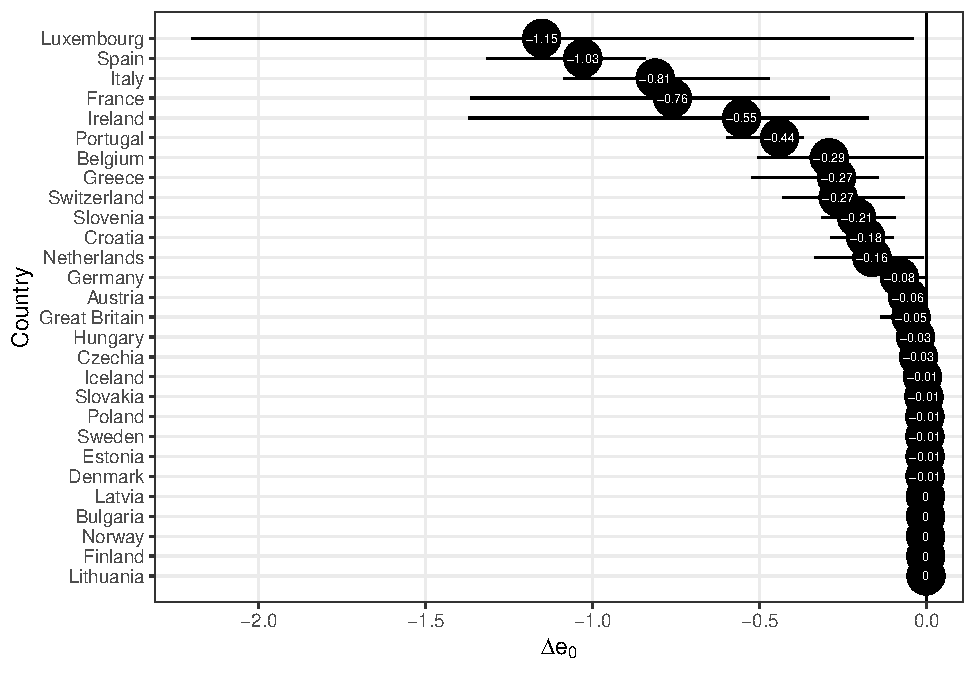
\includegraphics{MS-cclifeexpec_files/figure-latex/figure1-1.pdf}
\caption{Change in life expectancy at birth (\(e_0\)) due to
business-as-usual climate change in the 2080s compared to the present
\(e_0\). We report changes in life expectancies due to climate change
for twenty-eight European countries. The central values represent the
ensemble median while the stems represent the upper and lower bounds of
the inter-model climate variability.\label{figure1}}
\end{figure}

Our results also suggest climate change mortality differentials are
likely to unfold along highly uneven geographies (\autoref{map}).
Whereas many Northern European countries could experience negligible
impacts on life expectancy, five European countries could see life
expectancy changes in excess of -0.5 years (Spain, Luxembourg, France,
Italy, and Ireland). This group of countries could see life expectancy
changes of more than -1.0 years if climate change hazards are more
intense than anticipated. In some countries, climate change could thus
become a bigger killer than trachea, bronchus, and lung malignant
neoplasms (-0.85 years), acute myocardial infarction (-0.87 years), or
all accident related mortality (-0.84 years) (Arias et al. 2013) by the
end of the century.

\begin{figure}
\centering
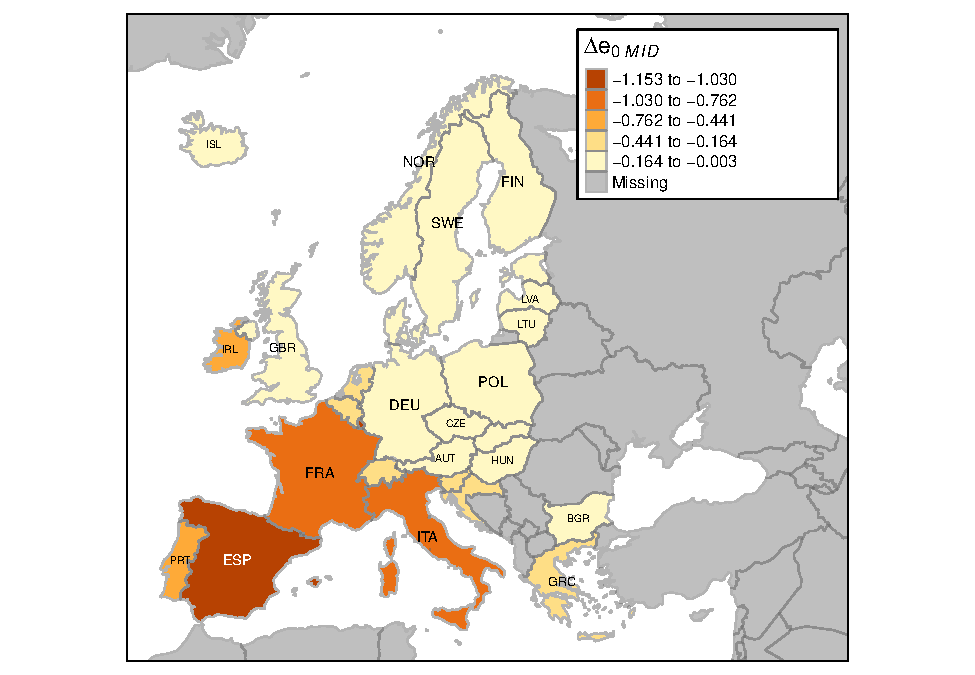
\includegraphics{MS-cclifeexpec_files/figure-latex/figure2-1.pdf}
\caption{Estimated reduction in life expectancy at birth (\(e_0\)) by
the 2080s under the \(MID\) scenario.\label{map}}
\end{figure}

While Forzieri et al's (Forzieri et al. 2017) results suggest that the
greatest climate change related mortality will unfold along a
north-south gradient, we find the greatest reduction in life expectancy
unfolds along an east-west gradient (\textbf{\autoref{map}}). The most
westerly European countries tend to have the greatest reductions.
Neighboring pairs of countries at similar latitudes could experience
vastly different mortality regimes, but neighboring pairs of countries
at similar longitudes seem to experience more similar mortality regimes
from climate change. Emergent research in Atmospheric Rivers suggest
Western Europe could be more susceptible to these types of events (Ramos
et al. 2015). Additionally, these results point to the importance of
converting excess mortality into life expectancy to properly quantify
the effects of climate change mortality.

\hypertarget{discussion}{%
\section{Discussion}\label{discussion}}

In this article, we demonstrate the impact climate change could have on
life expectancy at birth due to extreme weather events in twenty-eight
European countries. Previous studies on climate change and excess
mortality potentially miscommunicate the impact climate change could
have on human mortality. Contrary to excess mortality estimates, life
expectancy is routinely used as a primary metric for communicating
overall health outcomes and enjoys widespread use by major international
organizations (Marmot et al. 2012; Organization 2015; Salomon et al.
2012). Life expectancy and its derivatives are the recommended metrics
for population health (Parrish 2010). Additionally, it connects
mortality estimates into intuitively understandable metrics, translating
global estimates of mortality into personably relatable outcomes. Our
work reveals the extent to which climate change could reduce the average
person's longevity by the end of the century, expanding our
understanding of climate change and public health; thus linking two of
the major areas in current developmental and sustainability discussion
at both national and international levels (Abel et al. 2016).

Without adaptation measures, our results suggest climate change could
emerge as a significant new mortality vector and could pose a major
public health threat for some European countries by the end of the
century, echoing previous findings (Forzieri et al. 2017; Patz et al.
2005). Life expectancy has steadily risen across the world for the last
century (Gerland et al. 2014) and our results suggest that climate
change alone could spur a sharp reversal in these trends in some
countries. We expect two European countries to see life expectancy
reductions of more than one year under the middle scenario (Luxembourg
and Spain), but if climate change has a greater impact on mortality than
anticipated, five European countries (Luxembourg, Spain, Italy, France,
Ireland) could see life expectancy reductions of more than one year with
Luxembourg experiencing a reduction of more than two. These findings
highlight the hyperlocalized impacts of climate change (Forzieri et al.
2017; Kendon et al. 2014; Rosenzweig et al. 2010).

Reductions such as those should not be taken lightly. Many of the
children born today are likely to still be alive by the end of the
century and will be in the age groups (aged 65+) most threatened by the
biggest mortality risk associated with climate change (Keatinge et al.
2000) -- extreme heat. If climate change unfolds as a more aggressive
mortality vector, only all circulatory diseases combined or all cancers
combined would contribute more to mortality rates in numerous European
countries. This would make climate change one of the most aggressive new
mortality vectors to emerge over the last quarter-century, representing
a major threat to public health in many parts of Europe.

Prospective studies on the emerging threat from climate change rely on
linking contemporary mortality with future mortality. However, climate
change could reshape future mortality through other causes of death.
Climate change affects health behaviors that in turn increase mortality
risk through increased alcohol and substance abuse, violent behavior,
insecurity, increase in post-traumatic stress due to weather-related
trauma, increase in stress due to climate change and schizophrenia,
increase in the use of medications that reduce the ability to perspire
and sweat, etc. (Patz et al. 2005) The International Classifications of
Diseases and Related Health Problems (ICD) does not contain ``climate
change" as an official cause of death, so we can only speculate that the
impact of climate change could be larger than reported here. Although we
do not model these potential impacts, our results could thus be
considered conservative.

We also share the concerns of Lee et al. (Lee and Kim 2017) concerning
the business-as-usual climatic assumptions. It is likely that many
countries and communities will deploy a wide variety of adaptation
measures (Ebi, Kovats, and Menne 2006; Haines et al. 2006; Kovats et al.
2003). These adaptation measures rely on accurate information about the
potential mortality vectors. Our models and those produced by Forzieri
et al. (Forzieri et al. 2017) present plausible scenarios on the
potential impact of climate change on human mortality and provide
crucial information to public health officials, national governments,
and international organizations. The time frames associated with climate
change allow ample time for this potential health crisis to be averted.

These results should also be considered conservative when compared to
the broader impact of climate change on human longevity. The disaster
databases that Forzieri et al (Forzieri et al. 2017) use in generating
their excess mortality estimates probably, though the disaster databases
are unclear, only account for the deaths certified as \emph{directly}
caused by these hazards and are unlikely to capture the overall numbers
associated with these deaths. If the certification of deaths due to
weather extremes is similar to the certication in the present, than our
results and those of Forzieri et al reflect the exess mortality directly
attributable to climatic extremes. Despite this limitation, the impact
of these extremes on \(e_0\) is considerable, even if conservative.

Finally, we would like to point out that future research should not only
transform excess mortality into life expectancy decrements. Given the
influence of climate change in diseases and causes of death, it is
imperative to quantify the extent to which climate change will derive in
increasing costs for health care systems in these countries. The health
care structures are being taxed by population aging (Rechel et al. 2009)
and rising health care costs, yet it remains unclear how climate change
will exacerbate these pressures.

\newpage

\hypertarget{refs}{}
\leavevmode\hypertarget{ref-abel2016meeting}{}%
Abel, Guy J., Bilal Barakat, KC Samir, and Wolfgang Lutz. 2016.
``Meeting the Sustainable Development Goals Leads to Lower World
Population Growth.'' \emph{Proceedings of the National Academy of
Sciences} 113(50):14294--9.

\leavevmode\hypertarget{ref-arias2013united}{}%
Arias, Elizabeth, Melonie Heron, and Betzaida Tejada-Vera. 2013.
``United States Life Tables Eliminating Certain Causes of Death,
1999-2001.'' \emph{National Vital Statistics Reports: From the Centers
for Disease Control and Prevention, National Center for Health
Statistics, National Vital Statistics System} 61(9):1--128.

\leavevmode\hypertarget{ref-barnett2007climate}{}%
Barnett, Jon and W. Neil Adger. 2007. ``Climate Change, Human Security
and Violent Conflict.'' \emph{Political Geography} 26(6):639--55.

\leavevmode\hypertarget{ref-beltran2008integrated}{}%
Beltrán-Sánchez, Hiram, Samuel H. Preston, and Vladimir Canudas-Romo.
2008. ``An Integrated Approach to Cause-of-Death Analysis: Cause-Deleted
Life Tables and Decompositions of Life Expectancy.'' \emph{Demographic
Research} 19:1323.

\leavevmode\hypertarget{ref-cloyd2016engagement}{}%
Cloyd, Emily, Susanne C. Moser, Edward Maibach, Julie Maldonado, and
Tinqiao Chen. 2016. ``Engagement in the Third Us National Climate
Assessment: Commitment, Capacity, and Communication for Impact.''
\emph{Climatic Change} 135(1):39--54.

\leavevmode\hypertarget{ref-HMD}{}%
Database, Human Mortality. 2017. ``University of California, Berkeley
(Usa), and Max Planck Institute for Demographic Research (Germany).''
Available at www.mortality.org or www.humanmortality.de, (datadownloaded
on 1 August 2017).

\leavevmode\hypertarget{ref-GBD}{}%
Disease Study 2015, Global Burden of. 2017. ``Lobal Burden of Disease
Study 2015 (Gbd 2015) Results.'' Seattle, UnitedStates: Institute for
Health Metrics and Evaluation (IHME), 2016.Available from
http://ghdx.healthdata.org/gbd--results--tool.For terms and conditions
of use, pleasevisit
http://www.healthdata.org/about/terms--and--conditions.

\leavevmode\hypertarget{ref-ebi2006approach}{}%
Ebi, Kristie L., R. Sari Kovats, and Bettina Menne. 2006. ``An Approach
for Assessing Human Health Vulnerability and Public Health Interventions
to Adapt to Climate Change.'' \emph{Environmental Health Perspectives}
114(12):1930.

\leavevmode\hypertarget{ref-forzieri2017increasing}{}%
Forzieri, Giovanni, Alessandro Cescatti, Filipe Batista e Silva, and Luc
Feyen. 2017. ``Increasing Risk over Time of Weather-Related Hazards to
the European Population: A Data-Driven Prognostic Study.'' \emph{The
Lancet Planetary Health} 1(5):e200--e208.

\leavevmode\hypertarget{ref-gerland2014world}{}%
Gerland, Patrick, Adrian E. Raftery, Hana Ševčíková, Nan Li, Danan Gu,
Thomas Spoorenberg, Leontine Alkema, Bailey K. Fosdick, Jennifer Chunn,
Nevena Lalic, and others. 2014. ``World Population Stabilization
Unlikely This Century.'' \emph{Science} 346(6206):234--37.

\leavevmode\hypertarget{ref-haines2006climate}{}%
Haines, Andy, R. Sari Kovats, Diarmid Campbell-Lendrum, and Carlos
Corvalán. 2006. ``Climate Change and Human Health: Impacts,
Vulnerability and Public Health.'' \emph{Public Health} 120(7):585--96.

\leavevmode\hypertarget{ref-hsiang2017estimating}{}%
Hsiang, Solomon, Robert Kopp, Amir Jina, James Rising, Michael Delgado,
Shashank Mohan, DJ Rasmussen, Robert Muir-Wood, Paul Wilson, Michael
Oppenheimer, and others. 2017. ``Estimating Economic Damage from Climate
Change in the United States.'' \emph{Science} 356(6345):1362--9.

\leavevmode\hypertarget{ref-jiang2014internal}{}%
Jiang, Leiwen. 2014. ``Internal Consistency of Demographic Assumptions
in the Shared Socioeconomic Pathways.'' \emph{Population and
Environment} 35(3):261--85.

\leavevmode\hypertarget{ref-keatinge2000heat}{}%
Keatinge, WR, GC Donaldson, Elvira Cordioli, M. Martinelli, AE Kunst, JP
Mackenbach, S. Nayha, and I. Vuori. 2000. ``Heat Related Mortality in
Warm and Cold Regions of Europe: Observational Study.'' \emph{Bmj}
321(7262):670--73.

\leavevmode\hypertarget{ref-kendon2014heavier}{}%
Kendon, Elizabeth J., Nigel M. Roberts, Hayley J. Fowler, Malcolm J.
Roberts, Steven C. Chan, and Catherine A. Senior. 2014. ``Heavier Summer
Downpours with Climate Change Revealed by Weather Forecast Resolution
Model.'' \emph{Nature Climate Change} 4(7):570.

\leavevmode\hypertarget{ref-kovats2003methods}{}%
Kovats, RS, K. Ebi, Bettina Menne, Diarmid Campbell-Lendrum, OF
Canziani, A. Githeko, K. Kuhn, D. Le Sueur, P. Martens, AJ McMichael,
and others. 2003. \emph{Methods of Assessing Human Health Vulnerability
and Public Health Adaptation to Climate Change}. WHOHealth
CanadaUNEPWMO.

\leavevmode\hypertarget{ref-lee2017comprehensive}{}%
Lee, Jae Young and Ho Kim. 2017. ``Comprehensive Assessment of Climate
Change Risks.'' \emph{The Lancet Planetary Health} 1(5):e166--e167.

\leavevmode\hypertarget{ref-marmot2012building}{}%
Marmot, Michael, Jessica Allen, Ruth Bell, and Peter Goldblatt. 2012.
``Building of the Global Movement for Health Equity: From Santiago to
Rio and Beyond.'' \emph{The Lancet} 379(9811):181--88.

\leavevmode\hypertarget{ref-mcmichael2006climate}{}%
McMichael, Anthony J., Rosalie E. Woodruff, and Simon Hales. 2006.
``Climate Change and Human Health: Present and Future Risks.'' \emph{The
Lancet} 367(9513):859--69.

\leavevmode\hypertarget{ref-melillo2014climate}{}%
Melillo, Jerry M., TT Richmond, and G. Yohe. 2014. ``Climate Change
Impacts in the United States.'' \emph{Third National Climate
Assessment}.

\leavevmode\hypertarget{ref-o2017roads}{}%
O'Neill, Brian C., Elmar Kriegler, Kristie L. Ebi, Eric Kemp-Benedict,
Keywan Riahi, Dale S. Rothman, Bas J. van Ruijven, Detlef P. van Vuuren,
Joern Birkmann, Kasper Kok, and others. 2017. ``The Roads Ahead:
Narratives for Shared Socioeconomic Pathways Describing World Futures in
the 21st Century.'' \emph{Global Environmental Change} 42:169--80.

\leavevmode\hypertarget{ref-world2015world}{}%
Organization, World Health. 2015. \emph{World Health Statistics 2015}.
World Health Organization.

\leavevmode\hypertarget{ref-pachauri2014climate}{}%
Pachauri, Rajendra K., Myles R. Allen, Vicente R. Barros, John Broome,
Wolfgang Cramer, Renate Christ, John A. Church, Leon Clarke, Qin Dahe,
Purnamita Dasgupta, and others. 2014. \emph{Climate Change 2014:
Synthesis Report. Contribution of Working Groups I, Ii and Iii to the
Fifth Assessment Report of the Intergovernmental Panel on Climate
Change}. IPCC.

\leavevmode\hypertarget{ref-parrish2010peer}{}%
Parrish, R. Gibson. 2010. ``Peer Reviewed: Measuring Population Health
Outcomes.'' \emph{Preventing Chronic Disease} 7(4).

\leavevmode\hypertarget{ref-patz2005impact}{}%
Patz, Jonathan A., Diarmid Campbell-Lendrum, Tracey Holloway, and
Jonathan A. Foley. 2005. ``Impact of Regional Climate Change on Human
Health.'' \emph{Nature} 438(7066):310.

\leavevmode\hypertarget{ref-ramos2015daily}{}%
Ramos, Alexandre M., Ricardo M. Trigo, Margarida LR Liberato, and
Ricardo Tomé. 2015. ``Daily Precipitation Extreme Events in the Iberian
Peninsula and Its Association with Atmospheric Rivers.'' \emph{Journal
of Hydrometeorology} 16(2):579--97.

\leavevmode\hypertarget{ref-rechel2009can}{}%
Rechel, Berndl, Yvonne Doyle, Emily Grundy, Martin McKee, World Health
Organization, and others. 2009. ``How Can Health Systems Respond to
Population Ageing.''

\leavevmode\hypertarget{ref-rigaud2018groundswell}{}%
Rigaud, Kanta Kumari, Alexander M. De Sherbinin, Bryan Jones, Jonas
Bergmann, Viviane Clement, Kayly Ober, Jacob Schewe, Susana Beatriz
Adamo, Brent McCusker, Silke Heuser, and others. 2018. ``Groundswell:
Preparing for Internal Climate Migration.''

\leavevmode\hypertarget{ref-rosenzweig2010cities}{}%
Rosenzweig, Cynthia, William Solecki, Stephen A. Hammer, and Shagun
Mehrotra. 2010. ``Cities Lead the Way in Climate--Change Action.''
\emph{Nature} 467(7318):909.

\leavevmode\hypertarget{ref-salomon2012healthy}{}%
Salomon, Joshua A., Haidong Wang, Michael K. Freeman, Theo Vos, Abraham
D. Flaxman, Alan D. Lopez, and Christopher JL Murray. 2012. ``Healthy
Life Expectancy for 187 Countries, 1990--2010: A Systematic Analysis for
the Global Burden Disease Study 2010.'' \emph{The Lancet}
380(9859):2144--62.

\leavevmode\hypertarget{ref-samir2017human}{}%
Samir, KC and Wolfgang Lutz. 2017. ``The Human Core of the Shared
Socioeconomic Pathways: Population Scenarios by Age, Sex and Level of
Education for All Countries to 2100.'' \emph{Global Environmental
Change} 42:181--92.

\leavevmode\hypertarget{ref-wang2012age}{}%
Wang, Haidong, Laura Dwyer-Lindgren, Katherine T. Lofgren, Julie Knoll
Rajaratnam, Jacob R. Marcus, Alison Levin-Rector, Carly E. Levitz, Alan
D. Lopez, and Christopher JL Murray. 2012. ``Age-Specific and
Sex-Specific Mortality in 187 Countries, 1970--2010: A Systematic
Analysis for the Global Burden of Disease Study 2010.'' \emph{The
Lancet} 380(9859):2071--94.

\leavevmode\hypertarget{ref-wilson2017climate}{}%
Wilson, Ander, Brian J. Reich, Christopher G. Nolte, Tanya L. Spero,
Bryan Hubbell, and Ana G. Rappold. 2017. ``Climate Change Impacts on
Projections of Excess Mortality at 2030 Using Spatially Varying
Ozone--Temperature Risk Surfaces.'' \emph{Journal of Exposure Science
and Environmental Epidemiology} 27(1):118--24.

\leavevmode\hypertarget{ref-zanobetti2012summer}{}%
Zanobetti, Antonella, Marie S. O'neill, Carina J. Gronlund, and Joel D.
Schwartz. 2012. ``Summer Temperature Variability and Long-Term Survival
Among Elderly People with Chronic Disease.'' \emph{Proceedings of the
National Academy of Sciences} 109(17):6608--13.
\newpage
\singlespacing 
\end{document}